\documentclass[12pt]{article}
\usepackage[top = 1in,bottom=1.6in,left=1in,right=1in]{geometry}
\usepackage{titlesec}
\usepackage{setspace}
\usepackage{array}
\usepackage{graphicx}
\usepackage{amssymb}
\usepackage{hyperref}
\usepackage{xcolor}
\usepackage{listings}
\usepackage[english]{babel}
\usepackage{url}
\usepackage{makeidx}
\usepackage{graphicx}
\usepackage{lmodern}
\usepackage{hyperref}
\usepackage{url}


%%%%%%%%%% C code predefined settinngs start here %%%%%%%%%%%%%%%%%%%%%%%
%%%%%%%%%%%%%%%%%%%%%%%%%%%%%%%%%%%%%%%%%%%%%%%%%%%%%%%%%%%%%%%%%%%%%%%%%

\definecolor{mGreen}{rgb}{0,0.6,0}
\definecolor{mGray}{rgb}{0.5,0.5,0.5}
\definecolor{mPurple}{rgb}{0.58,0,0.82}
\definecolor{backgroundColour}{rgb}{0.95,0.95,0.92}

\lstdefinestyle{CStyle}{
    backgroundcolor=\color{backgroundColour},   
    commentstyle=\color{mGreen},
    keywordstyle=\color{magenta},
    numberstyle=\tiny\color{mGray},
    stringstyle=\color{mPurple},
    basicstyle=\footnotesize,
    breakatwhitespace=false,         
    breaklines=true,                 
    captionpos=b,                    
    keepspaces=true,                 
    numbers=left,                    
    numbersep=5pt,                  
    showspaces=false,                
    showstringspaces=false,
    showtabs=false,                  
    tabsize=2,
    language=C
}

%%%%%%%%% Program code predefined settings end here %%%%%%%%%%%%%%%%%%%%%%%%
%%%%%%%%%%%%%%%%%%%%%%%%%%%%%%%%%%%%%%%%%%%%%%%%%%%%%%%%%%%%%%%%%%%%%%%%%%%%

\begin{document}


%%%%%%%%% Front Page %%%%%%%%%%%%%%%%%%%%%%%%%%%%%%%%%%%%%%%%%%%%%%%%%%%%%%%
%%%%%%%%%%%%%%%%%%%%%%%%%%%%%%%%%%%%%%%%%%%%%%%%%%%%%%%%%%%%%%%%%%%%%%%%%%%%

\begin{center}
\textbf{Assignment 8 \\
\vspace{10mm}
ELP - 718 Telecom Software Laboratory \\
\vspace{5mm}
Kartik Gupta \\
\vspace{2mm}
2018JTM2250 \\
\vspace{2mm}
2018-2020} \\
\vspace{10mm}
A report presented for the assignment on \\
\vspace{2mm}
Python / Github

\vspace{30mm}

\includegraphics[scale=0.5]{logo.png} \\
\vspace{12mm}
\textbf{Bharti School Of} \\
\vspace{2mm}
\textbf{Telecommunication Technology and Management} \\
\vspace{2mm}
\textbf{IIT Delhi} \\
\vspace{2mm}
\textbf{India} \\
\vspace{2mm}
\textbf{September 27, 2018}

\end{center}

%%%%%%%%%%%%%%%%%%%%%%%%%%%%%%%%%%%%%%%%%%%%%%%%%%%%%%%%%%%%%%%%%%%%%%%%%%%%%%%%
%%%%%%%%%%%%%%%%%%%%%%%%%%%%%%%%%%%%%%%%%%%%%%%%%%%%%%%%%%%%%%%%%%%%%%%%%%%%%%%%

\newpage
\tableofcontents
\newpage
\listoffigures
\newpage


%%%%%%% Problem Statement 1 %%%%%%%%%%%%%%%%%%%%%%%%%%%%%%%%%%%%%%%%%%%%%%%%%%%%
%%%%%%%%%%%%%%%%%%%%%%%%%%%%%%%%%%%%%%%%%%%%%%%%%%%%%%%%%%%%%%%%%%%%%%%%%%%%%%%%

\section{Problem Statement-1}

\subsection{Problem Statement}
IIT Delhi, has just got the strongest computer. The professors in charge wants to check the computational capacity of the computer. So, they decided to create the problem which is to be given as an assignment to students. Can you help the professor to check the computation capability of the computer?\\
A valid cross is defined here as the two regions (horizontal and vertical) of equal lengths crossing over each other. These lengths must be odd, and the middle cell of its horizontalregion must cross the middle cell of its vertical region.\\

\begin{figure}[h]
\begin{center}
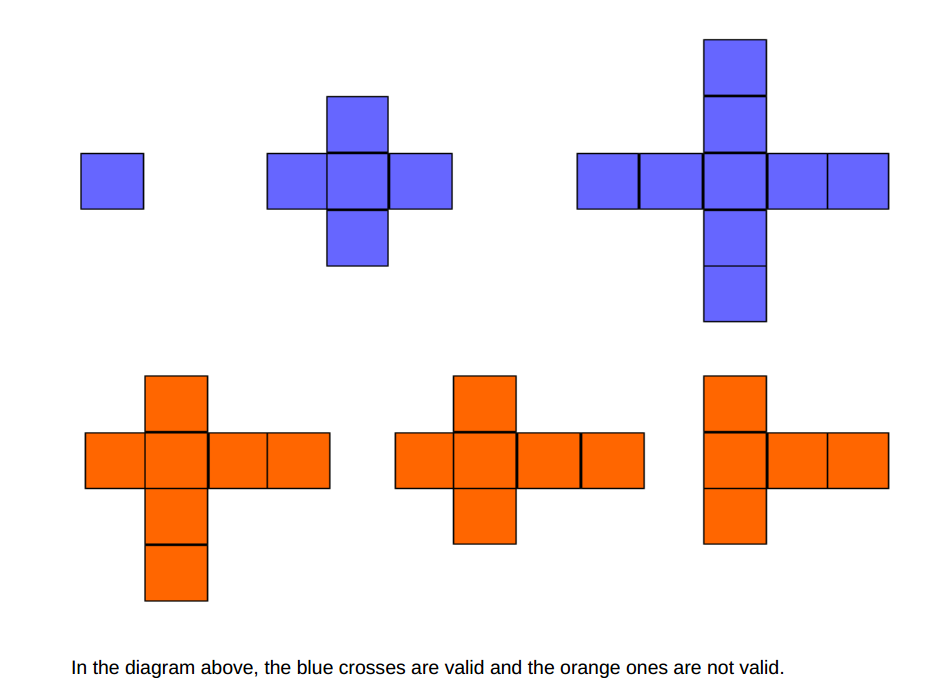
\includegraphics[scale=0.5]{dig.png}
\end{center}
\end{figure}


Find the two largest valid crosses that can be drawn on smart cells in the grid, and return two integers denoting the dimension of the each of the two largest valid crosses. In the above diagrams, our largest crosses have dimension of 1, 5 and 9 respectively .

\subsection{Input Format}
The first line contains two space-separated integers, n and m.\\
Each of the next lines n contains a string of m characters where each character is either S(Smart) or D (Dull). These strings represent the rows of the grid. If the jth character in the ith line is S, then (i,j) is a cell smart. Otherwise it's a dull cell.


\subsection{Output Format}
Find two valid crosses that can be drawn on smart cell of the grid, and return the dimension of both the crosses in the reverse sorted order(i.e. First Dimension should be the larger one and other should be smaller one).


\newpage
\subsection{Program Structure}
\begin{figure}[h]
\begin{center}
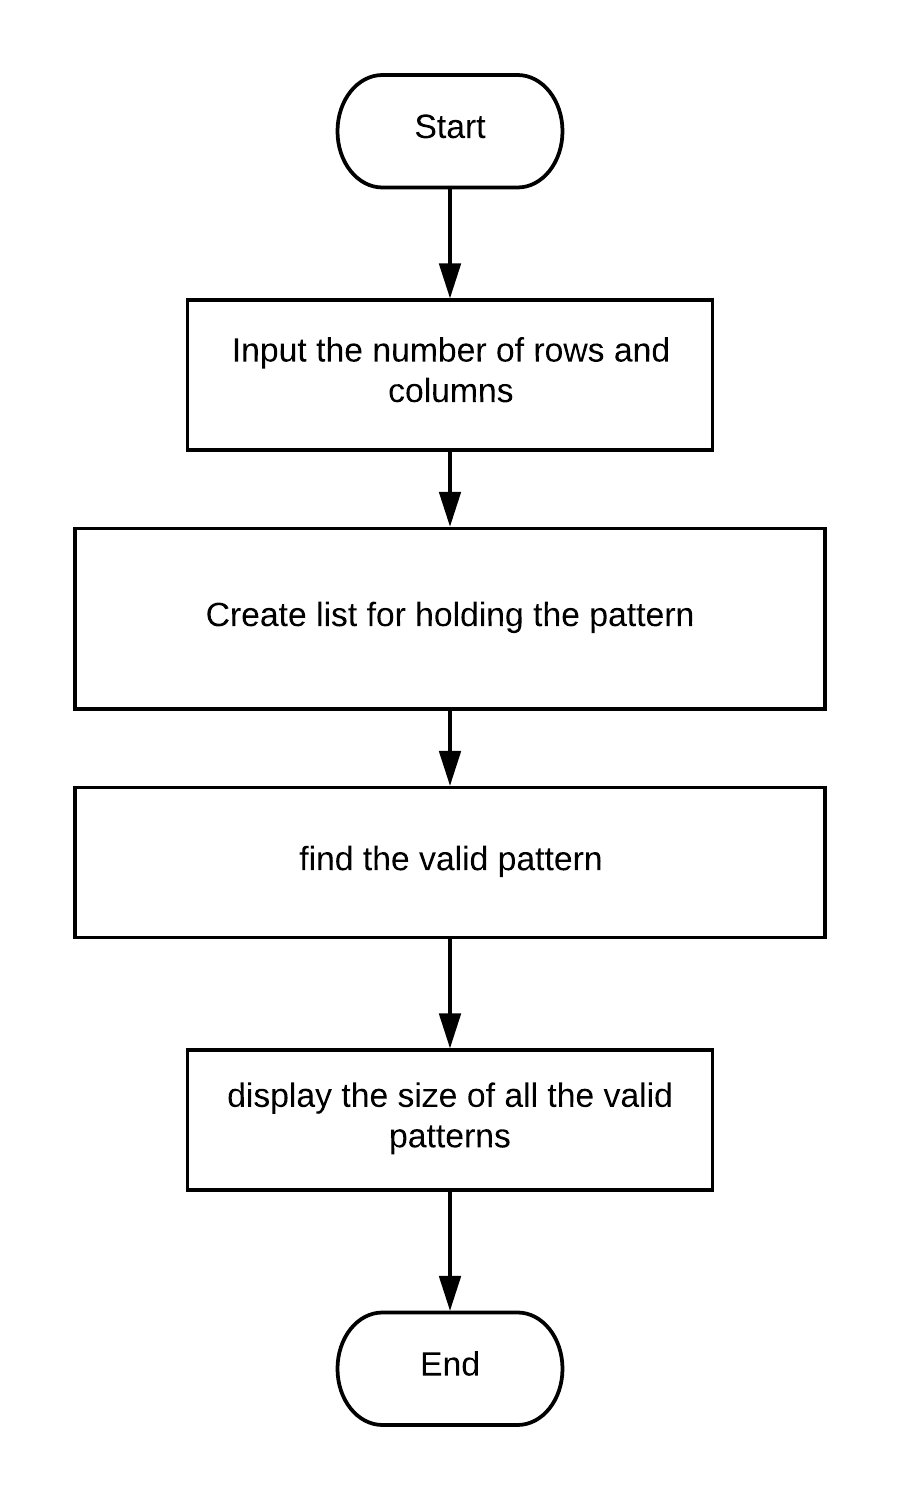
\includegraphics[scale=1.05]{ps1_fc.png}
\caption{Flowchart for Program 1}
\end{center}
\end{figure}

\newpage
\subsection{Algorithm and inmplementation}

\begin{itemize}
\item Input the number of rows and columns 
\item Create list for holding the pattern
\item find the valid pattern  
\item display the size of all the valid patterns
\end{itemize}


\subsection{TestCases}
\textbf{Sample Input 0}\\
5 6\\
SSSSSS\\
SDDDSD\\
SSSSSS\\
SSDDSD\\
SSSSSS\\
\textbf{Sample Output 0}\\
5 1


\subsection{Screenshots}
\begin{figure}[h]
\begin{center}
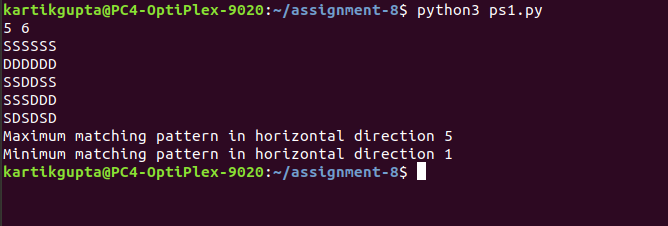
\includegraphics[scale=.7]{ps1_result.png}
\caption{Problem 1 Result}
\end{center}
\end{figure}
\newpage



%%%%%%% Problem Statement 2 %%%%%%%%%%%%%%%%%%%%%%%%%%%%%%%%%%%%%%%%%%%%%%%%%%%%
%%%%%%%%%%%%%%%%%%%%%%%%%%%%%%%%%%%%%%%%%%%%%%%%%%%%%%%%%%%%%%%%%%%%%%%%%%%%%%%%

\section{Problem Statement-2}

\subsection{Problem Statement}
After, getting mix results of valid crosses, professors decided to test the computation abilities on one more problem. This time professors wanted to test the decryption capabilities of the computer.\\
Encryption of a message requires three keys, k1, k2, and k3. The 26 letters of English and
underscore are divided in three groups, [a-i] form one group, [j-r] a second group, and
everything else ([s-z] and underscore) the third group. Within each group the letters are
rotated left by ki positions in the message. Each group is rotated independently of the other two. Decrypting the message means doing a right rotation by ki positions within each group.


\subsection{Input Format}
All input strings comprises of only lowercase English alphabets and underscores.

\subsection{Output Format}
For each encrypted message, the output is a single line containing the decrypted string.

\newpage
\subsection{Program Structure}

\begin{figure}[h]
\begin{center}
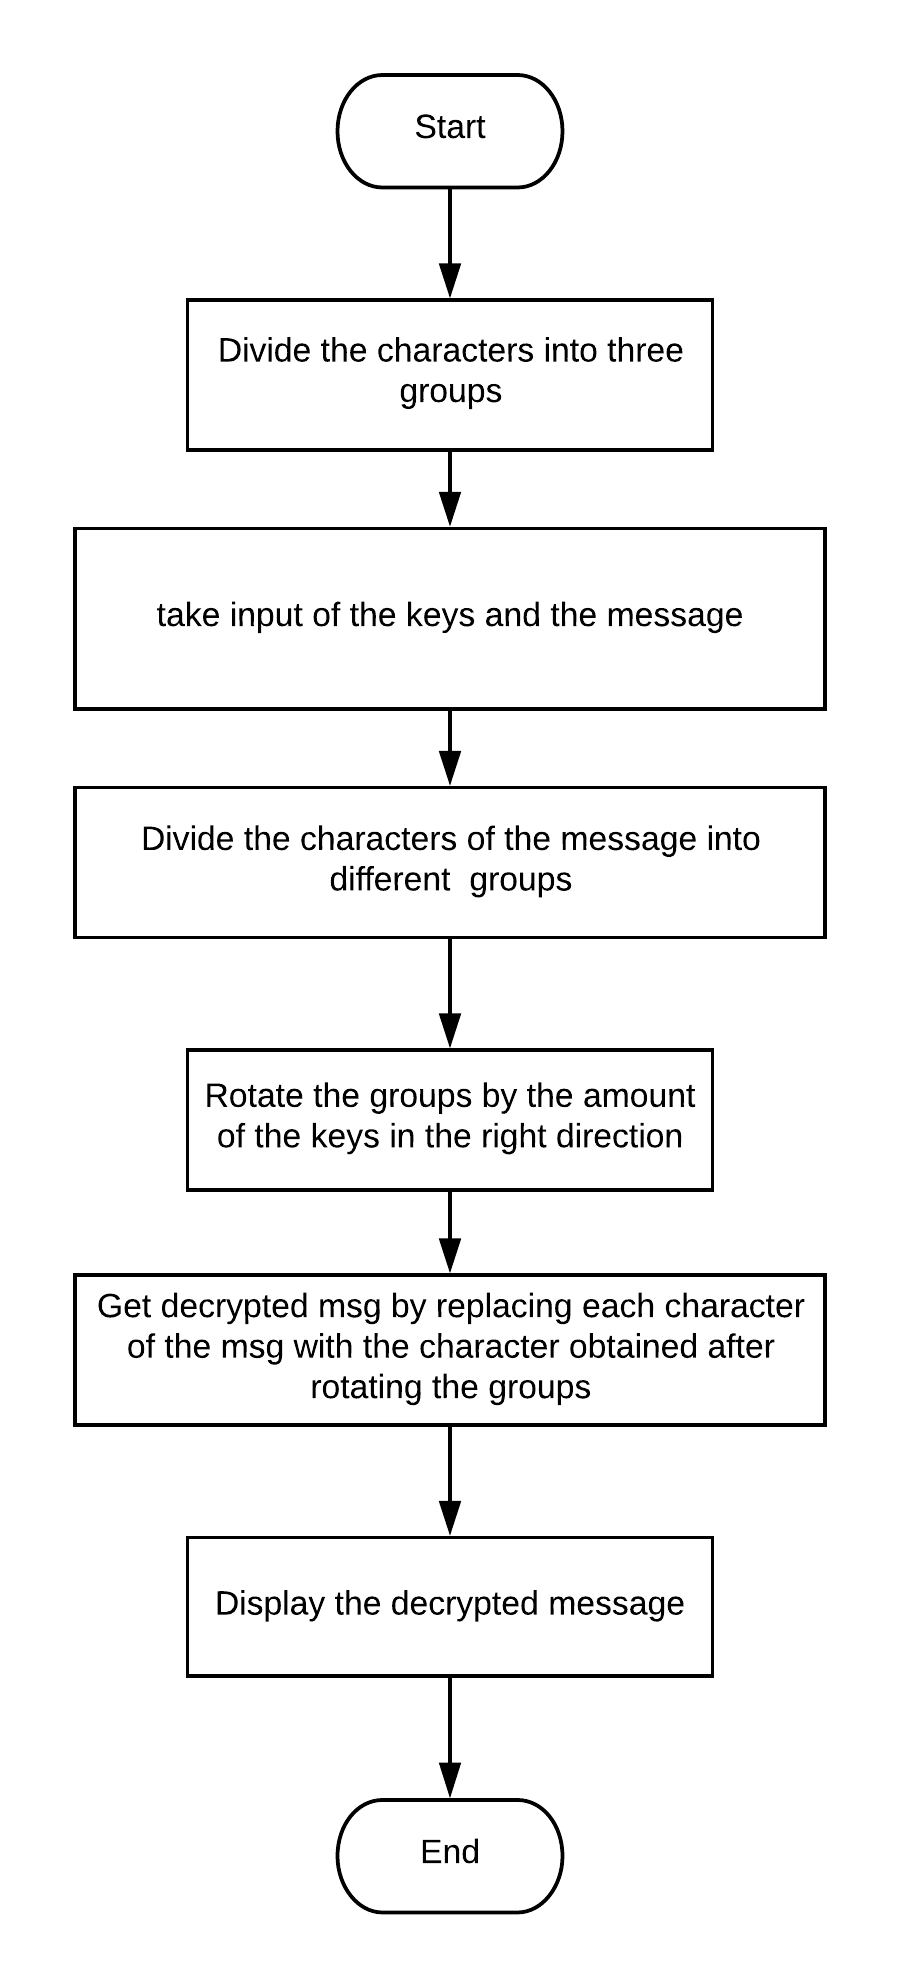
\includegraphics[scale=0.9]{ps2_fc.png}
\caption{Flowchart for Program 2}
\end{center}
\end{figure}

\newpage

\subsection{Algorithm and inmplementation}

\begin{itemize}
\item Divide the characters into three groups
\item  take input of the keys and the message
\item Divide the characters of the message into different  groups
\item Rotate the groups by the amount of the keys in the right direction
\item Get decrypted msg by replacing each character of the msg with the character obtained after rotating the groups
\item Display the decrypted message

\end{itemize}

\subsection{TestCases}
\textbf{Sample Input 0}\\
2 3 4\\
dikhtkor\_ey\_tec\_ocsusrsw\_ehas\_\\
\textbf{Sample Output 0}\\
hardwork\_is\_the\_key\_to\_success\\
\textbf{Sample Input }\\
1 1 1\\
bktcluajs\\
\textbf{Sample Output 1}\\
ajsbktclu


\newpage

\subsection{Screenshots}
\begin{figure}[h]
\begin{center}
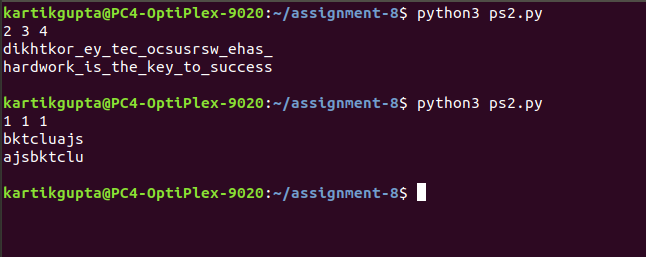
\includegraphics[scale=.70]{ps2_result.png}
\caption{Problem 2 Result}
\end{center}
\end{figure}
\newpage



\newpage



\section{Appendix}        
\subsection{Code for ps1.py}
\begin{lstlisting}[style=CStyle]

#
#  @file ps1.py
#
#  @author Kartik Gupta
#  @date 27 September 2018
#

# Getting number of rows and columns
r,c = list([int(i) for i in input().split()])
listarr=[]
listnew=[]
x=1

# Initializing lists for the pattern
for i in range(106):
     listarr.append('')

listnew=[]

# Getting characters for pattern
for i in range(r):
    si=input()
    l=list(si[:c])+['','','','','','','']
    listarr.insert(i,l)


for i in range(r):
    for j in range(c):
        if listarr[i][j]=="S":
            for k in range(1,c):
                if (listarr[i][j+k]=="S") and (listarr[i][j-k]=="S") :
                    x+=2

            listnew.append(x)
            x=1

maxvalue=max(listnew)
minvalue=min(listnew)
print("Maximum matching pattern in horizontal direction" +  " " + str(maxvalue))
print("Minimum matching pattern in horizontal direction" +  " " + str(minvalue))

\end{lstlisting}     
     
\newpage
     
\subsection{Code for ps2.py}
\begin{lstlisting}[style=CStyle]

#
#  @file ps2.py
#
#  @author Kartik Gupta
#  @date 27 September 2018
#

# Creating groups for different characters
group1 = list("abcdefghi")
group2 = list("jklmnopqr")
group3 = list("stuvwxyz_")

# initializing list for groups
gr1=[]
gr2=[]
gr3=[]
gr1new=[]
gr2new=[]
gr3new=[]

# initializing list for index
index1=[]
index2=[]
index3=[]

#Getting k1,k2 and k3 values
k1,k2,k3 = [int(i) for i in input().split()]

# getting input string
word=input()
wordlist=list(word)

# Dividing the characters into different groups
for i in range(len(word)):
    if wordlist[i] in group1:
        gr1.append(wordlist[i])
        index1.append(i)
    elif wordlist[i] in group2:
        gr2.append(wordlist[i])
        index2.append(i)
    elif wordlist[i] in group3:
        gr3.append(wordlist[i])
        index3.append(i)

# Rotating the groups
gr1new = (gr1[-k1:] + gr1[:-k1])
gr2new = (gr2[-k2:] + gr2[:-k2])
gr3new = (gr3[-k3:] + gr3[:-k3])

#Getting decrypted msg
p=q=r=0
for i in range(0,len(word)):
    if i in index1:
        wordlist[i]=gr1new[p]
        p+=1
    elif i in index2:
        wordlist[i]=gr2new[q]
        q+=1
    elif i in index3:
        wordlist[i]=gr3new[r]
        r+=1

#displaying the decrypted msg
for i in wordlist[:]:
    print (i, end ='')
    
print("\n")



\end{lstlisting}





\newpage


\nocite{*}
\bibliographystyle{plain}
\bibliography{referances.bib}


     


\end{document}